%\documentclass[a4paper,11pt]{book}
%\usepackage[spanish]{babel} % Para escribir en Espanol normal
%\usepackage[utf8]{inputenc}
%\usepackage[latin1]{inputenc}
%\usepackage{color}
%\usepackage{array}
%\usepackage{amsmath,amssymb}
%\usepackage{float}
%\usepackage{graphicx}
%\usepackage{subfig}
%\usepackage{enumerate}
%\usepackage{hyperref}%para hacer referencias

%\begin{document}

%Portada del Documento
\chapter{GitHub}
\setlength{\unitlength}{1 cm} %Especificar unidad de trabajo
\thispagestyle{empty}
\begin{picture}(10,10)
\put(3,0){
\includegraphics[width=8cm,height=10cm]{./imagenes1/apli1.png}}
\end{picture}
\begin{center}

\end{center}

% fin de la portada

\newpage


\section{ Introducción}

GitHub es un proyecto en linea que sirve para guardar tus proyectos utilizando el sistema de control de versiones Git. El codigo se almacena de forma pùblica o privada.
    \subsection{ Requisitos}
\begin{itemize}
\item  Abrir una cuenta en la pagina de GitHub
 \url{  http://www.github.com}
       \begin{figure}[htb]
\centering
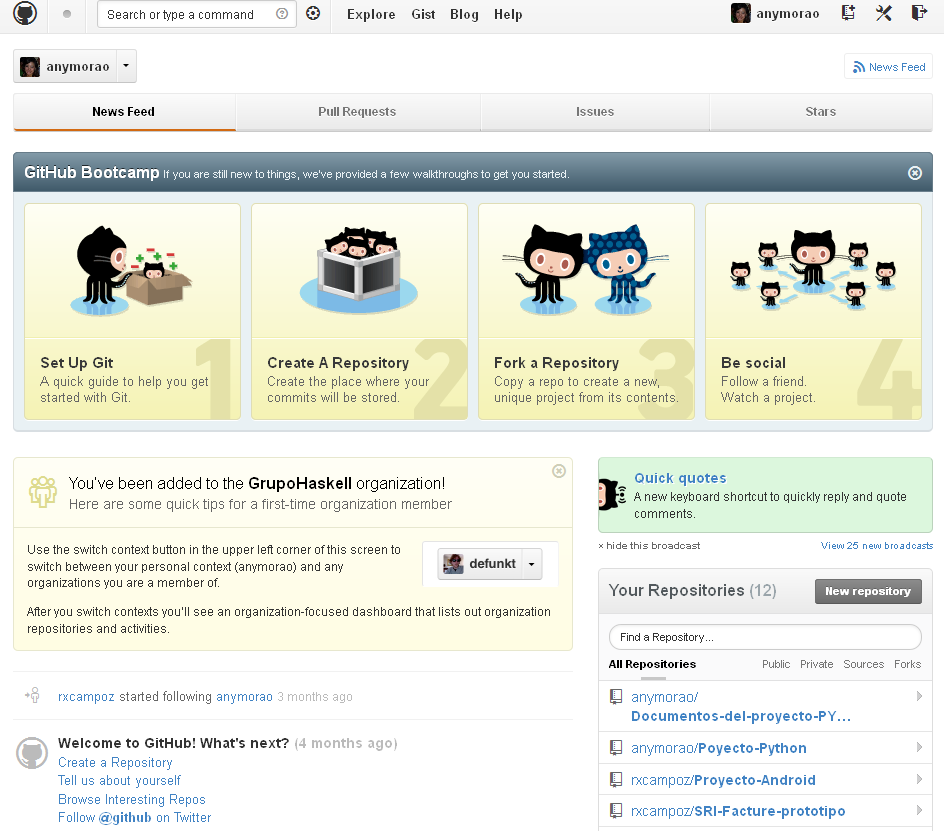
\includegraphics[width=0.77\textwidth]{./imagenes1/Dibujo1.png}
\end{figure}

 \item Instalar GitHub para window.
      \begin{figure}[htb]
\centering
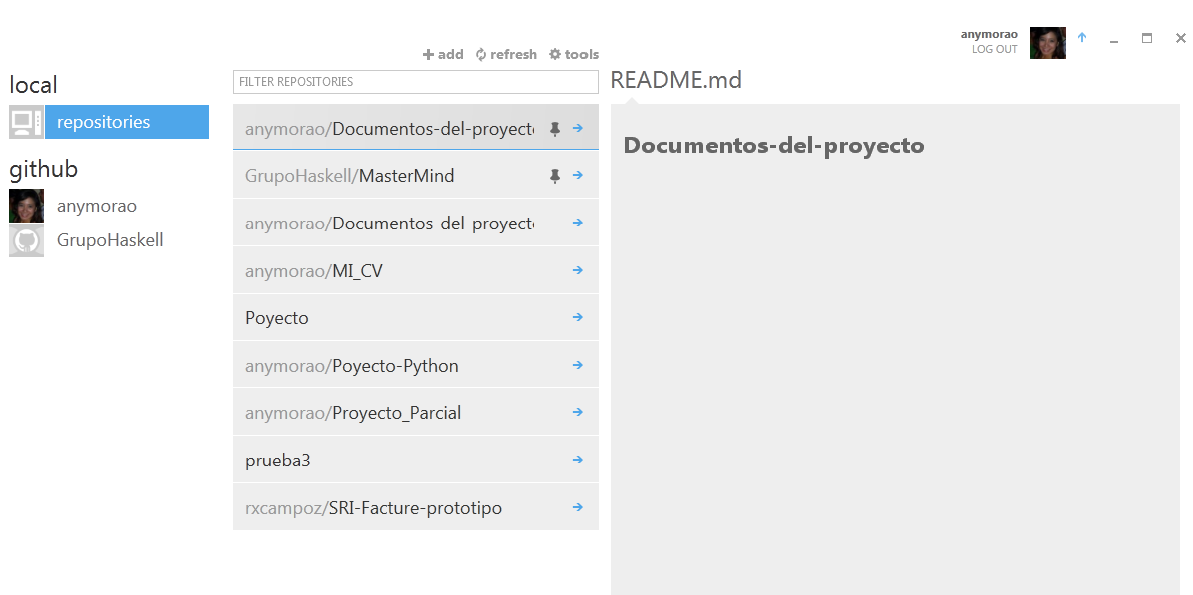
\includegraphics[width=0.77\textwidth]{./imagenes1/Dibujo2.png}
\end{figure}

 \item Crear el repositorio donde guardaras el proyecto.
     \begin{figure}[htb]
\centering
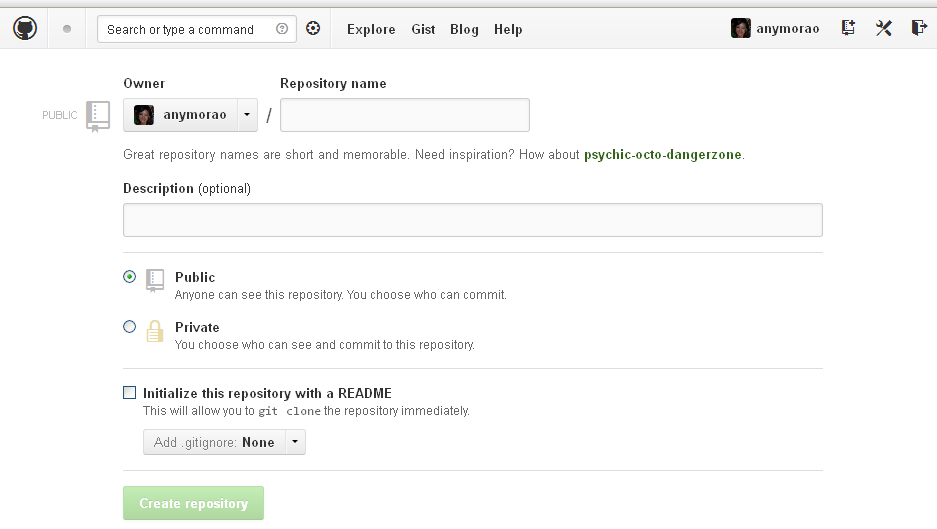
\includegraphics[width=0.87\textwidth]{./imagenes1/Dibujo3.png}
\end{figure}

\end{itemize}

 \section{ Experiencias}
\begin{itemize}
 \item Github fue dificil de manejar  para mi ya que no estava acostumbrada a tener un repositorio donde guaradar mis proyectos , intente instalar por consola y se me hizo muy dificil asi que opte por intarlar el github para windows aunque me tomò un tiempo aprender como usarlo pude lograrlo. 
 \item La falta de costumbre hace que me olvide de subir las versiones al github y cada vez que hago un cambio no lo guardo y subo el proyecto ya terminado.
\item Al principio no sabia como realizar un commit esa fue  una de las razones por la que no subia nada al GitHub asi que tuve que pedirle ayuda a un compañero, gracias a la paciensia que tuvo pa explicarme pude realizar un commit.
\end{itemize}

%\end {document}

